\PassOptionsToPackage{subsection=false}{beamerouterthememiniframes}
\documentclass[9pt,compress,t,aspectratio=169]{beamer}
\usetheme[
	bullet=circle,
	alternativetitlepage=true,
	titleline=true,
	titlepagelogo=img/sissa_and_mathlab,
]{mathlab}
\usepackage[utf8]{inputenc}
\usepackage[T1]{fontenc}
\usepackage[english]{babel}
\usepackage{amsmath}
\usepackage{amsthm}
\usepackage{amsfonts}
\usepackage{graphicx}
\usepackage{caption}
\usepackage{subcaption}
\usepackage{verbatim} % per comment
\usepackage{lmodern} % font più chiaro
\usepackage{ragged2e}
\usepackage{bm}
\usepackage{tikz}
\usepackage[thicklines]{cancel}
\usepackage{xcolor}
\usepackage{wasysym}
\usepackage{units}
\usepackage{tikzsymbols}
\usepackage{bbm}


\usepackage{multimedia}
\usepackage{graphicx}
\usepackage{pgfplots}
\usepackage{pgfplotstable}

\usetikzlibrary{shadows}

\usetikzlibrary{decorations.pathreplacing,calligraphy}

%\usepackage{media9}%
\newcommand\Ccancel[2][black]{\renewcommand\CancelColor{\color{#1}}\cancel{#2}}
\newcommand{\cfbox}[2]{%
    \colorlet{currentcolor}{.}%
    {\color{#1}%
    \fbox{\color{currentcolor}#2}}%
}



\newcommand{\bad}{\Sadey[2][red]}
\newcommand{\good}{\Smiley[2][green]}

\newcommand{\one}{$[1]$}
\newcommand{\two}{$[2]$}
\newcommand{\three}{$[3]$}


\setbeamertemplate{navigation symbols}{}


\graphicspath{%
	{images/}%
}


% \usepackage[normal]{subfigure}
\usepackage{amssymb}
\usepackage{color,xcolor,soul}
%\DeclareMathOperator{\supp}{supp}
\usepackage{mathrsfs}
\DeclareGraphicsExtensions{.pdf,.jpg,.png}
\usepackage{hyperref}
%\usepackage{algorithm2e}
\usepackage{comment}
\usepackage{algorithm,algorithmic}

\usetikzlibrary{arrows,chains,matrix,positioning,scopes}



\definecolor{green}{rgb}{0.0, 0.42, 0.14}
\definecolor{lightgreen}{rgb}{0,0.5,0}
\definecolor{lightblue}{rgb}{0.1,0.3,0.5}
\newcommand{\mathcolorbox}[2]{\colorbox{#1}{$\displaystyle #2$}}

\newcommand{\R}{\mathbb R}
\newcommand{\Z}{\mathbb Z}
\newcommand{\N}{\mathbb N}
\newcommand{\C}{\mathbb C}
\newcommand{\Q}{\mathbb Q}
\newcommand{\K}{\mathbb K}
\newcommand{\PP}{\mathbb P}
\newcommand{\TT}{\mathcal{T}}
\newcommand{\normal}{\mathbf{N}}

\renewcommand{\SS}{\mathcal{S}}
\newcommand{\KK}{\mathcal{K}}
\newcommand{\EE}{\mathcal{E}}

%%%%%Dante 
\newcommand{\diff}[1]{{\mathrm{d}{#1}}}
\newcommand{\dotprod}{\boldsymbol \cdot}
\newcommand{\ddt}[1]   {\frac{\partial{#1}}{\partial{t}}}
\newcommand{\dsddt}[1] {\dfrac{\partial{#1}}{\partial{t}}}
\newcommand{\txddt}[1] {\tfrac{\partial{#1}}{\partial{t}}}
\newcommand{\ddp}[2]   { \frac{\partial #1}{\partial #2}}
\newcommand{\dsddp}[2] {\dfrac{\partial #1}{\partial #2}}
\newcommand{\txddp}[2] {\tfrac{\partial #1}{\partial #2}}
\newcommand{\ddo}[2]   { \frac{\diff #1}{\diff #2}}
\newcommand{\dsdo}[2]  {\dfrac{\diff #1}{\diff #2}}
\newcommand{\txddo}[2] {\tfrac{\diff #1}{\diff #2}}
\newcommand{\Div}[1] { \boldsymbol{\nabla} \!\dotprod #1 }
\newcommand{\Grad}[1] { \boldsymbol{\nabla} #1 }
\newcommand{\Gradr}[1]{\widetilde{\boldsymbol{\nabla} {#1}}}
\newcommand{\vect}[1] {\boldsymbol{#1}}
\newcommand{\versor}[1] {\hat{ \boldsymbol{#1}}}
\newcommand{\vzero}{\boldsymbol{0}}
\newcommand{\IdxM} {\mathbb{I}}

 %----------------> Euler and NS equation
\newcommand{\vel}{\boldsymbol{v}}
\newcommand{\mm}{\boldsymbol{m}}
%\newcommand{\ee}{e}
\newcommand{\hh}{h}
\newcommand{\Et}{E^t}
\newcommand{\et}{e^t}
\newcommand{\qq}{\vect{q}}
\newcommand{\Rgas}{\mathcal{R}}
\newcommand{\vecu}{\mathsf{u}}
\newcommand{\vecf}{\boldsymbol{\mathsf{f}}}
\newcommand{\vecfa}{\boldsymbol{\mathsf{f}}^a}
\newcommand{\vecfv}{\boldsymbol{\mathsf{f}}^v}
\newcommand{\Jac}{\boldsymbol{\mathsf{A}}}   
\newcommand{\viscT}{\mathbb{S}}
\newcommand{\Kgas}{\kappa}

 %---------------> Numerical scheme
%\newcommand{\Rese}{{{\Phi}^e}}
%\newcommand{\Resei}{{{\Phi}^e_i}}
%\newcommand{\Reseib}{{{\Phi}^{f,\,\scriptscriptstyle{\partial}}_i}}
%\newcommand{\HResei}{{{\hat{\Phi}}^e_i}}
%\newcommand{\sHResei}{{{\hat{\Phi}}^{\,e, \star}_i}}
%\newcommand{\LResei}{{{\tilde{\Phi}}^e_i}}
%\newcommand{\vecw}{\mathsf{w}}
\newcommand{\ResKs}{{{\Phi}^K_\sigma}}
\newcommand{\ResK}{{{\Phi}^K}}
        
%---------------> Text style
\newcommand{\Tr}{\mathrm{T}}
\newcommand{\diag}{\mathop{\mathrm{diag}}}
\newcommand{\xx}{\boldsymbol{x}}
\newcommand{\dV}{\,\mathrm{d}\Omega}
\newcommand{\dS}{\,\mathrm{d}\partial\Omega}
\newcommand{\vecn}{\boldsymbol{\mathbf n}}
\newcommand{\Ndofe}{N^e_\mathrm{dof}}
\newcommand{\Ndim}{{N_\mathrm{dim}}}
\newcommand{\Neqn}{{N_\mathrm{eq}}}
\newcommand{\E}{\mathrm{E}}
\newcommand{\FF}{\boldsymbol{\mathsf{R}}} 
\newcommand{\JJ}{\mathbb{J}} 
\newcommand{\bbf}{{\mathbf {f}}}
\newcommand{\bxx}{{\mathbf {x}}}
\newcommand{\bn}{{\mathbf {n}}}
\newcommand{\s}{\sqrt{2}}
\newcommand{\is}{\frac{\sqrt{2}}{2}}
\newcommand{\hf}{\hat{f}}

\newcommand{\dpar}[2]{\dfrac{\partial #1}{\partial #2}}
\newcommand{\bu}{\mathbf{u}}
\newcommand{\bv}{\mathbf{v}}
\newcommand{\Bv}{\underline{\mathbf{v}}}
\newcommand{\bbv}{\mathbf{v}}
\newcommand{\Bbv}{\underline{\mathbf{v}}}
\newcommand{\bF}{\mathbf{F}}
\newcommand{\bFF}{\mathcal{F}}
\newcommand{\bbF}{\mathbf{\mathcal{F}}}
\newcommand{\bK}{\mathbf{K}}
\newcommand{\bbu}{\mathbf{u}}
\newcommand{\bbg}{\mathbf{g}}
\newcommand{\hbbg}{\hat{\mathbf{g}}}
\newcommand{\hbbf}{\hat{\mathbf{f}}}
\newcommand{\hbbfe}{\hat{\mathbf{f}}_{\sigma,\sigma'}}
\newcommand{\ba}{\mathbf{a}}
\newcommand{\bx}{\mathbf{x}}
\newcommand{\by}{\mathbf{y}}
\newcommand{\red}[1]{\textcolor{red}{#1}}
\newcommand{\blue}[1]{\textcolor{blue}{#1}}
\newcommand{\ICI}{\red{\large{ICI}}}

% ---- Notation Philipp
\newcommand{\bs}{\boldsymbol}
\renewcommand{\div}{\operatorname{div}}
\newcommand{\est}[1]{\left\langle#1\right\rangle}
\newcommand{\bU}{\mathbf{U}}
\newcommand{\bH}{\mathbf{H}}
\newcommand{\dd}{\mathrm{d}}
\newcommand{\bV}{\mathbf{V}}
\newcommand{\mean}[1]{\overline{#1}}
\newcommand{\bbfh}{{\mathbf {f}^h}}
\newcommand{\Ol}{\mathcal{O}}
\newcommand{\WW}{\mathrm{W}}
\newcommand{\LL}{\mathcal{L}}
\newcommand{\II}{\hat{I}_0}
\newcommand{\1}{\begin{pmatrix}
                 1\\
                 1
                \end{pmatrix}}
\newcommand{\e}[1]{\mathrm{e^{#1}}}
\newcommand{\VV}{\mathcal{V}}
\newcommand{\gnum}{g^{\operatorname{num}}}


%Numerical schemes
\newcommand{\Resjr}{\Phi^{j+\frac{1}{2}}_j}
\newcommand{\Resjl}{\Phi^{j-\frac{1}{2}}_j}

\newcommand{\Resjrn}{\Phi^{j+\frac{1}{2},n}_j}
\newcommand{\Resjln}{\Phi^{j-\frac{1}{2},n}_j}



\renewcommand{\vec}[1]{\underline{#1}}
%\NewDocumentCommand{\mat}{mo}{%
%  \IfValueTF{#2}{%
%    \underline{\underline{#1}}{#2}
%  }{%
%    \underline{\underline{#1}}\,
%  }%
%}
%Davide
\def\L{\mathcal{L}}
\def\I{\mathcal{I}}
\def\R{\mathbb{R}}
\def\bbc{\underline{\mathbf{c}}}
\def\bc{\mathbf{c}}
\def\bd{\mathbf{d}}
\def\bP{\mathbf{P}}
\def\bD{\mathbf{D}}
\def\bE{\mathbf{E}}
\def\bbd{\underline{\mathbf{d}}}
\def\M{\mathrm{M}}
\usepackage{bbm}

%Colors 
\definecolor{darkspringgreen}{rgb}{0., 0.55, 0.3}
\definecolor{dartmouthgreen}{rgb}{0.05, 0.5, 0.06}
\definecolor{etonblue}{rgb}{0.59, 0.78, 0.64}
\definecolor{airforceblue}{rgb}{0., 0.4, 0.66}
\definecolor{arylideyellow}{rgb}{0.91, 0.84, 0.42}
\definecolor{emerald}{rgb}{0.31, 0.78, 0.47}
\definecolor{uclagold}{rgb}{1.0, 0.7, 0.0}
\definecolor{cadmiumorange}{rgb}{0.93, 0.53, 0.18}




%%Shorten for Entropy function
%\newcommand{\Ucof}[2]{U_{(#1)}^{(#2)}}
%\newcommand{\Vcof}[2]{\bv_{(#1)}^{(#2),T}}
%\newcommand{\ecof}[2]{\eta_{(#1)}^{(#2)}}

%% Corrections
%\newcommand{\rev}[1]{\textcolor{red}{#1}}
%\newcommand{\revPP}[1]{\textcolor{blue}{#1}}
%\newcommand{\revDD}[1]{\textcolor{brown}{#1}}
%\newcommand{\revDP}[1]{\textcolor{darkspringgreen}{#1}}

\title[mPDeC modified Patankar Deferred Correction]{Arbitrary high-order,
 conservative and positive preserving\\
 Patankar-type deferred correction schemes} 

\author[D. Torlo]{\bf \Large Davide Torlo}

\institute[SISSA mathLab]{%
\vspace{-4mm}\\%
\small MathLab, Mathematics Area, SISSA International School for Advanced Studies, Trieste, Italy\\
\href{https://www.davidetorlo.it}{\underline{davidetorlo.it}}\vspace{-3mm}
}

\date[]
{ \small Based on: Öffner, P. \& Torlo, D. 
\textit{Arbitrary high-order, conservative and positivity preserving Patankar-type deferred correction schemes.} 
APNUM 153, 15--34 (2020). \url{https://doi.org/10.1016/j.apnum.2020.01.025}
}

\AtBeginSection[]
{
	\begin{frame}<beamer>
	\frametitle{Outline}
	  \tableofcontents[currentsection]
  
	\end{frame}


}

\begin{document}

\begin{frame}

\titlepage



\end{frame}

\begin{frame}<beamer>
	\frametitle{Outline}
	  \tableofcontents
  % You might wish to add the option [pausesections]
\end{frame}

\section{Production--Destruction system}
\begin{frame}{Production--Destruction system}

Consider {\color{lightgreen}production-destruction} systems (PDS) 
\begin{equation}\label{eq:original_model}
\begin{cases}
d_t c_i = P_i(\bc ) - D_i(\bc ) , \quad  i=1,\dots,I,\quad & P_i(\bc) = \sum_{j=1}^I p_{i,j}(\bc),\\
\bc(t=0)=\bc_0,& D_i(\bc) = \sum_{j=1}^I d_{i,j}(\bc),
\end{cases}
\end{equation}
where
$$p_{i,j}(\bc) , d_{i,j} (\bc) \geq 0, \qquad \forall i,j \in I, \quad \forall \bc \in \R^{+,I}.$$

\only<1>{Applications: Chemical reactions, biological systems, population evolutions and PDEs.\\ Example: SIRD
		\begin{equation*}
\begin{cases}
d_tS = - \beta \frac{SI}{N}\\
d_t I = \beta \frac{SI}{N} -\gamma I- \delta I \\
d_t R = \gamma I\\
d_t D = \delta I
\end{cases}
\end{equation*}}
\only<2>{Property 1: {\color{lightgreen}Conservation }
	\begin{align*}
		&\sum_{i=1}^I c_i(0) = \sum_{i=1}^I c_i(t), \quad \forall t\geq 0 \\
		\Longleftrightarrow \quad &p_{i,j}(\bc)=d_{j,i} (\bc) , \qquad \forall i,j \in I, \quad \forall \bc \in \R^{+,I}. \end{align*}}
\only<3>{Property 2: {\color{lightgreen}Positivity }
\begin{align*}
&\text{If }P_i,D_i\text{ Lipschitz, and if when } c_i\to 0 \Rightarrow D_i(\bc)\to 0 \Longrightarrow \\
&c_i(0) > 0 \,   \forall i \in I \Longrightarrow c_i(t)>0 \,\forall i \in I\; \forall t >0.
\end{align*}}
\only<4>{Goal: 
\begin{itemize}
\item One step method
\item Unconditionally positive
\item Unconditionally conservative
\item High order accurate
\end{itemize}
}
\end{frame}

\begin{frame}{Solvers}
	\begin{minipage}{0.45\textwidth}
\begin{block}{Explicit Euler}
\begin{itemize}
\item $\bc^{n+1}= \bc^n +\Delta t \left( \bP(\bc^n) -\bD(\bc^n) \right)$
\item Conservative 
\item First order
\item Not unconditionally positive, if $\Delta t$ is too big... CFL conditions
\end{itemize}
\end{block}
	\end{minipage} \hfill
\begin{minipage}{0.49\textwidth}
\begin{block}{Implicit Euler}
\begin{itemize}
	\item $
	\bc^{n+1}= \bc^n +\Delta t \left( \bP(\bc^{n+1}) -\bD(\bc^{n+1})\right)
	$
	\item Conservative \& positive
	\item First order
	\item Expensive to be solved/not unique solution: Nonlinear solvers!!!
\end{itemize}
\end{block}
\end{minipage}
\begin{block}{Patankar trick}
	\begin{minipage}{0.48\textwidth}
\vspace*{-2mm}\begin{equation*}
\begin{split}
c_i^{n+1}= c_i^n +\Delta t \left( P_i(\bc^{n}) -D_i(\bc^{n}){\color{lightgreen}\frac{c_i^{n+1}}{c_i^n}}\right) \\
\left( 1+\Delta t \frac{D_i(\bc^n)}{\color{lightgreen}c_i^n} \right){\color{lightgreen} c_i^{n+1}} = c^n_i +\Delta t P_i(\bc^{n}) 
\end{split}
\end{equation*}
	\end{minipage}\hfill
\begin{minipage}{0.45\textwidth}
\begin{itemize}
	\item Not conservative
	\item First order
	\item Positive
	\item Implicit, but easy
\end{itemize}
\end{minipage}
\end{block}

\end{frame}

\begin{frame}{Solvers}
Modified Patankar (mP)

Burchard, Deleersnijder \& Meister
\begin{equation}
\begin{split}
c_i^{n+1}= c_i^n +\Delta t \left( \sum_{j} p_{i,j} (\bc^{n}) {\color{lightblue}\frac{c_j^{n+1}}{c_j^n}} -\sum_j d_{i,j}(\bc^{n}){\color{lightgreen}\frac{c_i^{n+1}}{c_i^n}}\right )
\end{split}
\end{equation}
$\M(\bc^n) \bc^{n+1}=\bc^n$ where $\M$ is
\begin{equation}\label{eq:mass_matrix_mod_patankar}
\begin{cases}
m_{i,i}(\bc^n) = 1+\Delta t \sum_{k=1}^I {\color{lightgreen}\frac{d_{i,k}(\bc^n)}{c_i^n}} , \quad i=1,\dots, I,\\
m_{i,j}(\bc^n) = - \Delta t {\color{lightblue}\frac{p_{i,j}(\bc^n)}{c_j^n}} , \quad i,j=1,\dots , I ,\, i\neq j.
\end{cases}
\end{equation}
\begin{minipage}{0.4\textwidth}
\begin{itemize}
\item Conservative
\item First order
\item Positive
\item Linear system at each timestep
\end{itemize}
\end{minipage}\,
\begin{minipage}{0.58\textwidth}
	\begin{itemize}
		\item Extension to RK2 and RK3 (Burchard, Deleersnijder, Meister, Kopecz)
		\item Extension to PDEs (Huang, Zhao, Shu)
	\end{itemize}
\end{minipage}
%\begin{comment}
%\only<2-4>{ 
%\begin{align}
%\sum_i c_i^{n+1} = \sum_i c_i^n \only<2-3>{ + \Delta t \left( \sum_{i,j} p_{i,j}(\bc^n)\frac{c_j^{n+1}}{c_j^n} -\only<2>{\sum_{i,j} d_{i,j}(\bc) \frac{c_i^{n+1}}{c_i^n}}  \only<3>{\sum_{j,i} d_{j,i}(\bc) \frac{c_j^{n+1}}{c_j^n}}  \right) } 
%\end{align}
%}
%\only<5>{
%\item Positive
%\begin{itemize}
%\item $M$ is diagonal dominant by columns
%\item D the diagonal of M. Using the Jacobi method, we have that the iterative matrix to get to inverse of $M$ is defined as $(I-D^{-1}M)>0$
%\item $M^{-1}>0 $
%\end{itemize}
%}
%\end{comment}

\end{frame}


\section{Deferred Correction}
\begin{frame}{Deferred Correction discretization}
We should discretize our variable on $[t^n, t^{n+1}]$ in $M$ substeps ($\bc^{n,m}$).
\begin{figure}[ht]
	\centering
	\begin{tikzpicture}
\draw [thick]   (0,0) -- (7.5,0) node [right=2mm]{};
% nodes
\fill[black]    (0,0) circle (1mm) node[below=2mm] {$\only<1>{t^n} \only<2->{t^0} $} node[above=2mm] {$\only<1>{\bc^n} \only<2->{\bc^0}$}
(1.5,0) circle (0.7mm) node[below=2mm] {$\visible<2->{t^1}$} node[above=2mm] {$\visible<2->{\bc^1}$}
(3,0) circle (0.7mm) node[below=2mm] {}
(4.5,0) circle (0.7mm) node[below=2mm] {$\visible<2->{t^m}$} node[above=2mm] {$\visible<2->{\bc^m}$}
(6,0) circle (0.7mm) node[below=2mm] {}
(7.5,0) circle (1mm) node[below=2mm] {$\only<1>{t^{n+1}} \only<2->{t^M}$} node[above=2mm] {$\only<1>{\bc^{n+1}} \only<2->{\bc^M}$}; 
\end{tikzpicture} \caption{Subtimeintervals}\label{Fig:Time_interval}
\end{figure}
Then, we can rewrite $\bc^{m} = \bc^{0} + \int_{t^0}^{t^{m}} \bP (\bc(s)) -\bD(\bc(s))\, ds$.\\
Equispaced points $\Rightarrow $ order $=M+1$. \\
\begin{align}\label{eq:definition_bbc}
&\bbc :=  (\bc^0, \dots, \bc ^M) \in \R^{M\times I}%, \text{ such that }\\
%&\L^1(\bbc) := \L^1(\bc^0, \dots, \bc^M) \text{ and } \L^2(\bbc) := \L^2(\bc^0, \dots, \bc^M) .
\end{align}

\end{frame}
\begin{frame}{DeC operators}
\begin{minipage}{0.48\textwidth}
\begin{block}{$\L^2$ operator}
\only<1>{\begin{align*}
	&\bE:=\bP-\bD\\
&\L^2(\bc^0, \dots, \bc^M)=\L^2(\bbc) :=\\
&\begin{cases}
\bc^M-\bc^0 -{\color{lightgreen}\int_{t^0}^{t^M} \bE(\bc(s))ds}\\
\vdots\\
\bc^1-\bc^0 - \int_{t^0}^{t^1} \bE(\bc(s))ds
\end{cases}
\end{align*}}
\only<2->{
\begin{align*}
&\L^2(\bc^0, \dots, \bc^M)=\L^2(\bbc) :=\\
&\begin{cases}
\bc^M-\bc^0 - {\color{lightgreen}\Delta t \displaystyle\sum_{r=0}^M \theta_r^M \bE(\bc^r)}\\
\dots\\
\bc^1-\bc^0 - \Delta t \displaystyle\sum_{r=0}^M \theta_r^1 \bE(\bc^r)
\end{cases}
\end{align*}
}
\vspace*{-2mm}\begin{itemize}
	\item Implicit RK \item Order of accuracy $\geq M+1$ \item Difficult to solve directly
	\end{itemize}
\end{block}
\end{minipage}\hfill
\begin{minipage}{0.46\textwidth}
\only<3>{\begin{block}{$\L^1$ operator}
		\begin{align*}
			&\L^1(\bc^0, \dots, \bc^M) =\L^1(\bbc):=\\
			&\begin{cases}
			\bc^M-\bc^0 - {\color{lightgreen}\Delta t \beta^M \bE(\bc^0)} \\
			\dots\\
			\bc^1- \bc^0 - \Delta t \beta^1 \bE(\bc^0)
			\end{cases}
		\end{align*}
\begin{itemize}
	\item First order accurate
	\item Explicit or easy to solve
\end{itemize}
	\end{block}}
\end{minipage}

\end{frame}


\begin{frame}{Deferred Correction}
How to combine two methods keeping the accuracy of the second and the stability and simplicity of the first one?

\begin{minipage}{0.58\textwidth}
\begin{equation*}\label{DeC_method}
\begin{split}
&\bc^{0,(k)}:=\bc(t^n), \quad k=0,\dots, K,\\
&\bc^{m,(0)}:=\bc(t^n),\quad m=1,\dots, M\\
&\L^1(\bbc^{(k)})=\L^1(\bbc^{(k-1)})-\L^2(\bbc^{(k-1)})\text{ with }k=1,\dots,K.
\end{split}
\end{equation*}

\begin{block}{DeC Theorem}
	\begin{itemize} \item $\L^1$ coercive \item $\L^1-\L^2$ Lipschitz \end{itemize}
DeC converges and $\min(K,M+1)$ is the order of accuracy.
\end{block}
\end{minipage} \hfill
\begin{minipage}{0.4\textwidth}
	\begin{itemize}
		{
			\item $\mathcal{L}^1(\bbc)=0$, first order accuracy, easily invertible.
			\item $\mathcal{L}^2(\bbc)=0$, high order $M+1$.
		}
	\end{itemize}
	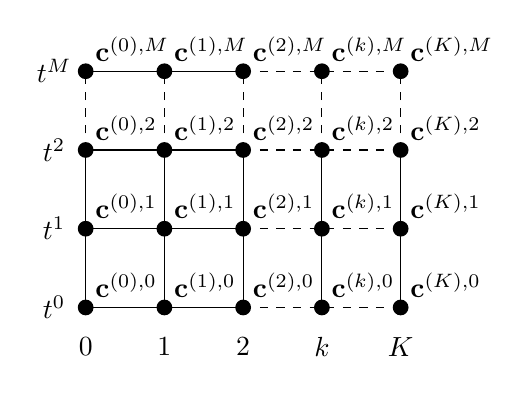
\begin{tikzpicture}
	\tikzset{dot/.style={fill=black,circle}}
	
	\foreach\l[count=\y] in {0,1,2,M}
	{
		\draw (1,\y) -- (3,\y);
		\draw[dashed] (3,\y) -- (5,\y);
		\node at (0.6,\y){$t^{\l}$};
		\foreach\foreach\z[count=\x] in {0,1,2,k,K}
		{
			\only<\x>{\fill (\x,\y) circle (1mm) node[anchor=south west] {$\bc^{(\z),\l}$};}
		}
	}
	
	\foreach\l[count=\x] in {0,1,2,k,K}
	{
		\draw (\x,1) -- (\x,3);
		\draw[dashed] (\x,3) -- (\x,4);
		\node at (\x,0.5){$\l$};
	}
		
	\end{tikzpicture}
\end{minipage}

\end{frame}

\begin{frame}{Explicit DeC}
If we write explicitly the DeC step we see that 

\begin{equation}
\begin{split}
\L^{1,m}_i(\bbc^{(k)}) &= \L^{1,m}_i(\bbc^{(k-1)})- \only<2>{\mathcolorbox{yellow}}{\L^{2,m}_i(\bbc^{(k-1)})} \Longleftrightarrow \\
c_i^{(k),m}\!\!\! - {\color{lightgreen}c_i^{0}} \!- {\color{lightblue}\Delta t \beta^m E_i(\bc^{0})} &= {\color{red}c_i^{(k-1),m}} - {\color{lightgreen}c_i^{0}} - {\color{lightblue}\Delta t \beta^m E_i(\bc^{0})} \\
& \,- {\color{red}c_i^{(k-1),m}} + c_i^{0} + \only<2>{\mathcolorbox{yellow}}{\Delta t \sum_{r=0}^M \theta^m_r E_i(\bc^{(k-1),r})} \Longleftrightarrow \\
c_i^{(k),m} &= c_i^{0} + \Delta t \sum_{r=0}^M \theta^m_r E_i(\bc^{(k-1),r}) \Longleftrightarrow \\
c_i^{(k),m} &= c_i(t^n) + \only<2>{\mathcolorbox{yellow}}{\Delta t \sum_{r=0}^M \theta^m_r E_i(\bc^{(k-1),r})}
\end{split}
\end{equation}

\end{frame}

\begin{frame}{Ingredients}
\begin{itemize}
\item We want to use the {\color{lightgreen}DeC for high order accuracy}
\item We want to recast {\color{lightgreen}positivity and conservation}
\item We will use the {\color{lightgreen}Patankar trick}
\item We want an implicit method (to get positivity), but only {\color{lightgreen}linearly implicit} (no nonlinear solvers)
\item We have to {\color{lightgreen}modify $\L^2$}  using the trick
\end{itemize}

\end{frame}

\section{Modified Patankar DeC (mPDeC)}
\begin{frame}{Modified Patankar $\L^2$}
Modify the operator $\L^2$ according to the Patankar trick!
\begin{equation*}\label{eq:L2m}
\!\!\begin{split}
&\L_i^2(\bc^{0,(k-1)}, \dots, \bc^{M,(k-1)}\visible<2->{,\bc^{0,(k)}, \dots, \bc^{M,(k)}}) =\L_i^2(\bbc^{(k-1)}\visible<2->{,\bbc^{(k)}}):=\\
&\begin{cases}
c_i^{M,(k-1)} \!\!\!-c_i^{0,(k-1)}\!\! -\Delta t \sum\limits_{r=0}^M {\color{red}\theta_r^M}  \! \sum\limits_{j=1}^I \!\! \left(   p_{i,j}(\bc^{r,(k-1)}) {\color{lightblue}\visible<2->{\frac{c^{M,(k)}_{\only<2>{j}\only<3>{\gamma(j,i, \theta_r^M)}}}{c_{\only<2>{j}\only<3>{\gamma(j,i, \theta_r^M)}}^{M,(k-1)}}}} -  d_{i,j}(\bc^{r,(k-1)})  \visible<2->{{\color{lightgreen}\frac{c^{M,(k)}_{\only<2>{i}\only<3>{\gamma(i,j, \theta_r^M)}}}{c_{\only<2>{i}\only<3>{\gamma(i,j, \theta_r^M)}}^{M,(k-1)}}}} \right),\\
\vdots\\
c_i^{1,(k-1)}-c_i^{0,(k-1)} \!\!- \Delta t  \sum\limits_{r=0}^M {\color{red}\theta_r^1} \sum\limits_{j=1}^I \!\!
\left(  p_{i,j}(\bc^{r,(k-1)}) \visible<2->{{\color{lightblue}\frac{c^{1,(k)}_{\only<2>{j}\only<3>{\gamma(j,i, \theta_r^1)}}}{c_{\only<2>{j}\only<3>{\gamma(j,i, \theta_r^1)}}^{1,(k-1)}}}} -  d_{i,j}(\bc^{r,(k-1)})  \visible<2->{{\color{lightgreen}\frac{c^{1,(k)}_{\only<2>{i}\only<3>{\gamma(i,j, \theta_r^1)}}}{c_{\only<2>{i}\only<3>{\gamma(i,j, \theta_r^1)}}^{1,(k-1)}}}} \right),
\end{cases}
\end{split}
\end{equation*}
\visible<3>{where $\gamma(a,b, \theta) = a$ if $\theta>0$ and $\gamma(a,b, \theta) = b$ if $\theta <0$.}
\end{frame}

\begin{frame}{Modified Patankar DeC (mPDeC)}
Reminder: initial states $c_i^{0,(k)}$ are identical for any correction $(k)$\\
DeC Patankar can be rewritten for $k=1,\dots,K$, $m =1,\dots, M$ and $\forall i\in I$ into

\begin{equation}\label{eq:explicit_dec_correction} 
\begin{split}
&\L^{1,m}_i (\bbc^{(k)})-\L^{1,m}_i (\bbc^{(k-1)})+\L^{2,m}_i (\bbc^{(k)},\bbc^{(k-1)})=0\\
&c_i^{m,(k)}-c^0_i -\Delta t   \sum_{r=0}^M \theta_r^m \sum_{j=1}^I 
\left( p_{i,j}(\bc^{r,(k-1)}) 
\frac{c^{m,(k)}_{\gamma(j,i, \theta_r^m)}}{c_{\gamma(j,i, \theta_r^m)}^{m,(k-1)}}
- d_{i,j}(\bc^{r,(k-1)})  \frac{c^{m,(k)}_{\gamma(i,j, \theta_r^m)}}{c_{\gamma(i,j, \theta_r^m)}^{m,(k-1)}} \right)=0.
\end{split}
\end{equation}
\begin{itemize}
\item Conservation
\item Positivity
\item High order accuracy
\end{itemize}

\end{frame}

\begin{frame}{Conservation}
The  mPDeC scheme is unconditionally conservative for all substages, 
i.e., $$\sum_{i=1}^I c^{m,(k)}_i=\sum_{i=1}^I c^{0}_i,$$ for all $k=1,\dots, K$ and $m=0,\dots,M$.

Using formulation \eqref{eq:explicit_dec_correction}, we can easily see that $\forall k,m$ 
\begin{align*}
&\sum_{i\in I} c_i^{m,(k)} - \sum_{i\in I} c_i^{0} =  \\
\only<1>{=&\Delta t \sum_{i,j=1}^I \sum_{r=0}^M \theta_r^m\left(
 {\color{red}p_{i,j}(\bc^{r,(k-1)})} \frac{c^{m,(k)}_{\gamma(j,i, \theta_r^m)}}{c_{\gamma(j,i, \theta_r^m)}^{m,(k-1)}} - d_{i,j}(\bc^{r,(k-1)})  \frac{c^{m,(k)}_{\gamma(i,j, \theta_r^m)}}{c_{\gamma(i,j, \theta_r^m)}^{m,(k-1)}} 
 \right) = }
\only<2>{ =&\Delta t \sum_{i,j=1}^I \sum_{r=0}^M\theta_r^m \left(
 {\color{red}d_{j,i}(\bc^{r,(k-1)})} \frac{c^{m,(k)}_{\gamma(j,i, \theta_r^m)}}{c_{\gamma(j,i, \theta_r^m)}^{m,(k-1)}} - d_{i,j}(\bc^{r,(k-1)})  \frac{c^{m,(k)}_{\gamma(i,j, \theta_r^m)}}{c_{\gamma(i,j, \theta_r^m)}^{m,(k-1)}} 
 \right) = }
 \only<3>{=&\Delta t \sum_{i,j=1}^I \sum_{r=0}^M\theta_r^m \left(
 {\color{red}d_{i,j}(\bc^{r,(k-1)})} \frac{c^{m,(k)}_{\gamma(i,j, \theta_r^m)}}{c_{\gamma(i,j, \theta_r^m)}^{m,(k-1)}} - d_{i,j}(\bc^{r,(k-1)})  \frac{c^{m,(k)}_{\gamma(i,j, \theta_r^m)}}{c_{\gamma(i,j, \theta_r^m)}^{m,(k-1)}} 
 \right) = 0.} 
\end{align*}
\end{frame}

\begin{frame}{Positivity}
At each step $(m,k)$ implicit linear system with mass matrix 
\begin{equation*}\label{eq:mass_matrix}
\begin{split}
&\M(\bc^{m,(k-1)})_{ij}= \\
&\!\begin{cases}
1+\Delta t \sum\limits_{r=0}^M \sum\limits_{l=1}^I  \frac{\theta_r^m}{c_i^{m,(k-1)}}   \left( {\color{lightgreen} d_{i,l}(\bc^{r,(k-1)})  \chi_{\lbrace \theta^m_r>0\rbrace}}  -{\color{lightblue} p_{i,l} (\bc^{r,(k-1)})\chi_{\lbrace \theta^m_r<0 \rbrace}} \right)  \,&\text{for }i=j\\
-\Delta t \sum\limits_{r=0}^M \frac{\theta_r^m}{c_j^{m,(k-1)}} \left({\color{lightblue}  p_{i,j}(\bc^{r,(k-1)})\chi_{\lbrace \theta^m_r>0\rbrace}} -{\color{lightgreen} d_{i,j} (\bc^{r,(k-1)})\chi_{\lbrace \theta^m_r<0\rbrace}} \right)  \, &\text{for }i\ne j
\end{cases}
\end{split}
\end{equation*}

\begin{itemize}
\item Diagonally dominant by columns
\item Invertible
\item $\M^{-1}>0$
\end{itemize}

\end{frame}

%\begin{frame}{Mass matrix}
%\begin{algorithm}
%	\fontsize{10pt}{10pt}\selectfont
%	\caption{Mass} 
%	\begin{algorithmic}[1]
%		{\REQUIRE Production-destruction functions $p_{i,j}(\cdot),\,d_{i,j}(\cdot)$, previous correction variables $\bbc^{(k-1)}$, actual subtimestep $m$.
%		\STATE $\M:=0$
%		\FOR{$i=1 $ \TO $ I$}
%			\FOR{$j=1$ \TO $I$}
%				\FOR{$r=0$ \TO $M$}
%					\IF{$\theta_r^m\geq 0$}
%						\STATE $\M_{i,j} = \M_{i,j} -\Delta t \theta_r^m \frac{p_{i,j}(\bc^{r,(k-1)})}{c_j^{m,(k-1)}}$
%						\STATE $\M_{i,i} = \M_{i,i} +\Delta t \theta_r^m \frac{d_{i,j}(\bc^{r,(k-1)})}{c_i^{m,(k-1)}}$
%					\ELSE
%						\STATE $\M_{i,j} = \M_{i,j} +\Delta t \theta_r^m \frac{d_{i,j}(\bc^{r,(k-1)})}{c_j^{m,(k-1)}}$
%						\STATE $\M_{i,i} = \M_{i,i} -\Delta t \theta_r^m \frac{p_{i,j}(\bc^{r,(k-1)})}{c_i^{m,(k-1)}}$	
%					\ENDIF
%				\ENDFOR
%			\ENDFOR
%		\ENDFOR
%		}
%	\end{algorithmic}\label{algo:mass}
%\end{algorithm}
%
%\end{frame}

\begin{frame}{High order accuracy}
Let $\bbc^*$ be the solution of the $\L^2$ operator, i.e., $\L^2(\bbc^*,\bbc^*)=0$.
\begin{itemize}
\item Coercivity operator $\L^1$: $||\L^1(\bbc)-\L^1(\bbc^*) ||\geq C_1||\bbc -\bbc^*||$ 
\item Lipschitz continuity operator $\L^1 - \L^2$:\\
$||\L^1 (\bbc^{(k-1)}) -\L^2 (\bbc^{(k-1)}, \bbc^{(k)}) -\L^1 ( \bbc^*) +\L^2 (\bbc^*,\bbc^*)||\leq C_L \Delta t ||\bbc^{(k-1)} -\bbc^*|| .$

\vspace{5mm}
Intermediate steps for Lipschitz continuity
\begin{itemize}
\item $
\bc^{m,(k)}=\bc^0 + \Delta t G(\bc^{m,(k-1)}) \bc^0
$
\item  $
  \frac{c_i^{(k)}}{c_i^{(k-1)}} =1+\Delta t^{k-1}g_i +\Ol(\Delta t^k)
 $
\end{itemize}

\end{itemize}

\end{frame}

\begin{frame}{Proof of DeC}
\begin{align}
||\bbc^{(k)}-\bbc^*||\leq & C_0|| \L^1(\bbc^{(k)}) - \L^1(\bbc^*) ||= \label{eq:coercivity}\\
= & C_0|| \L^1(\bbc^{(k-1)}) -\L^2(\bbc^{(k-1)}, \bbc^{(k)}) - \L^1(\bbc^*) +\L^2(\bbc^*, \bbc^*) ||\leq \label{eq:same_states}\\
\leq & C \Delta t || \bbc^{(k-1)}- \bbc^* || \label{eq:lipschitz}
\end{align}
After $K$ iterations 
%We can see that after $K$ iterations we have that the error decayed of a factor $\Delta t^K$, i.e., 
\begin{equation}
||\bbc^{(K)}-\bbc^*||\leq C^K \Delta t^K ||\bbc^0 -\bbc^*||.
\end{equation}

\end{frame}

\section{Numerics}
\begin{frame}{Linear test}
\begin{equation}\label{eq:linear_test}
\begin{aligned}
 &c_1'(t)=c_2(t)-5c_1(t),\quad  &c_2'(t)=5c_1(t)-c_2(t),\\
 &c_1(0)=c_1^0=0.9, \quad  &c_2(0)=c_2^0=0.1 \, .
\end{aligned}
\end{equation}
with
\begin{equation*}
  p_{1,2}(\bc)=d_{2,1}(\bc)=c_2, \quad p_{2,1}(\bc)=d_{1,2}(\bc)=5c_1 
\end{equation*}
and $p_{i,i}(\bc)=d_{i,i}(\bc)=0$ for $i=1,2$.

Analytical solution is
\begin{equation}\label{eq:analytical}
 c_1(t)=\frac{1}{6}\left(1 +  \frac{22}{5} \exp(-6t) \right) \text{ and } c_2(t)=1-c_1(t).
\end{equation}

\end{frame}

\begin{frame}{Linear test}
\begin{figure}[!htp]
\centering
    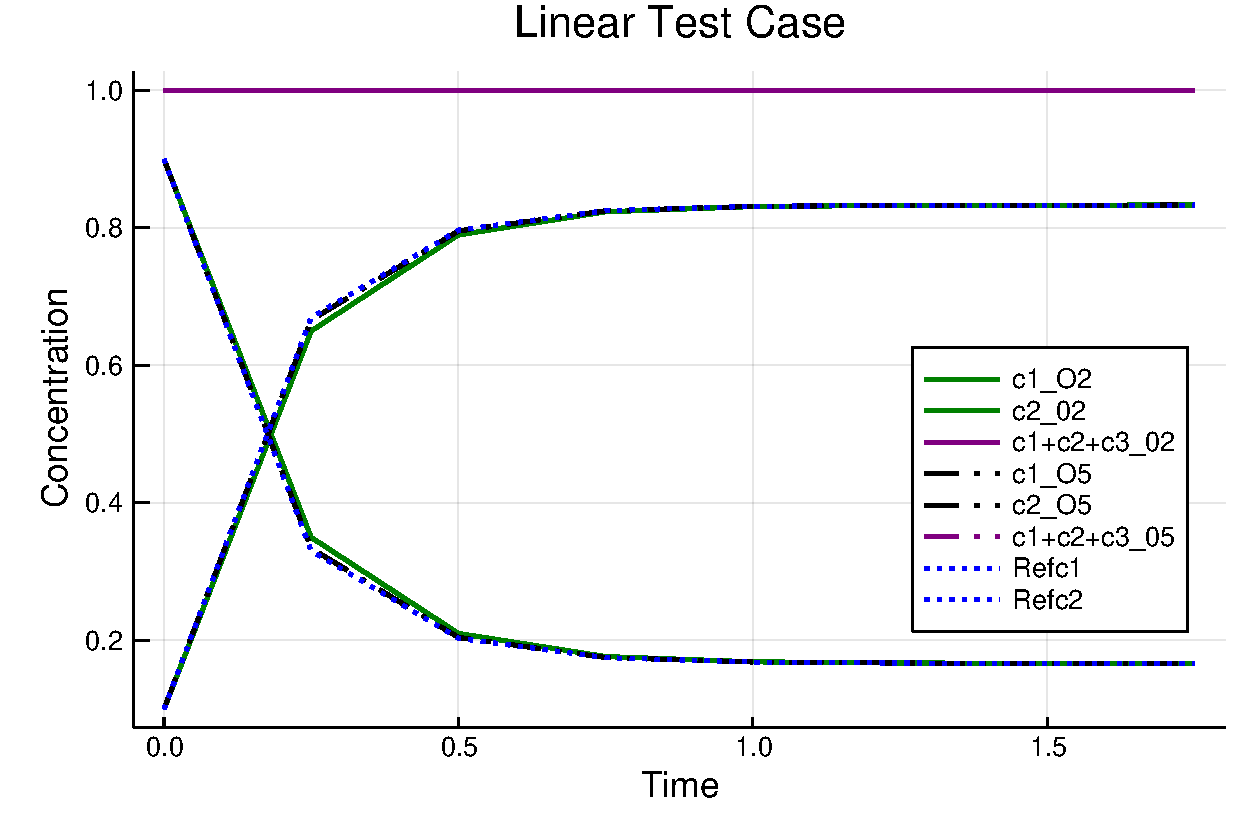
\includegraphics[height=0.7\textheight]{images/LinearOrder25.pdf}
  %  \includegraphics[width=0.45\textwidth]{Figures/Nonlinear/WithReference_DP.pdf}
  \caption{ Second and fifth order methods together with the reference solution \eqref{eq:analytical}
 }
  \label{fig:Linear_model}
\end{figure}

\end{frame}

\begin{frame}{Linear test: Convergence}
\begin{figure}[!htp]
\centering
    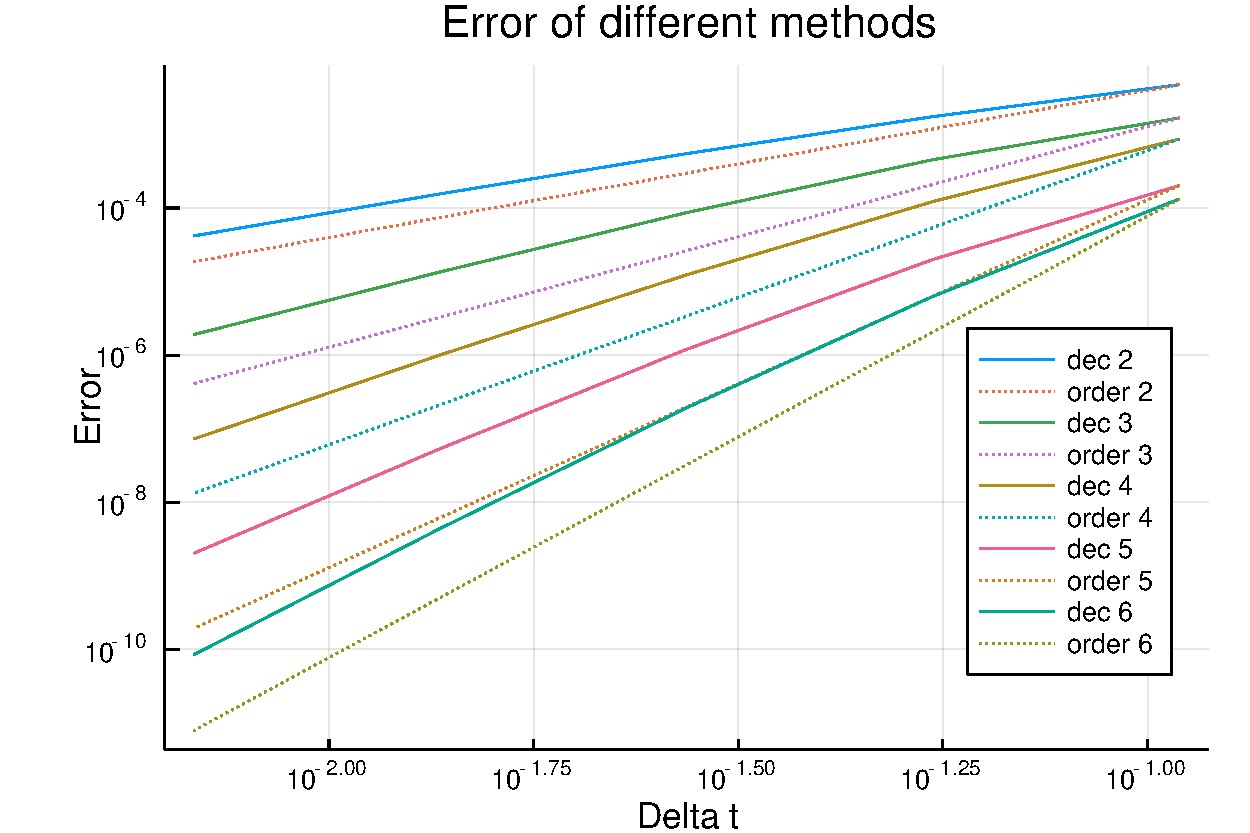
\includegraphics[width=0.48\textwidth]{images/LinearIntegralErrorOrders26.pdf}
    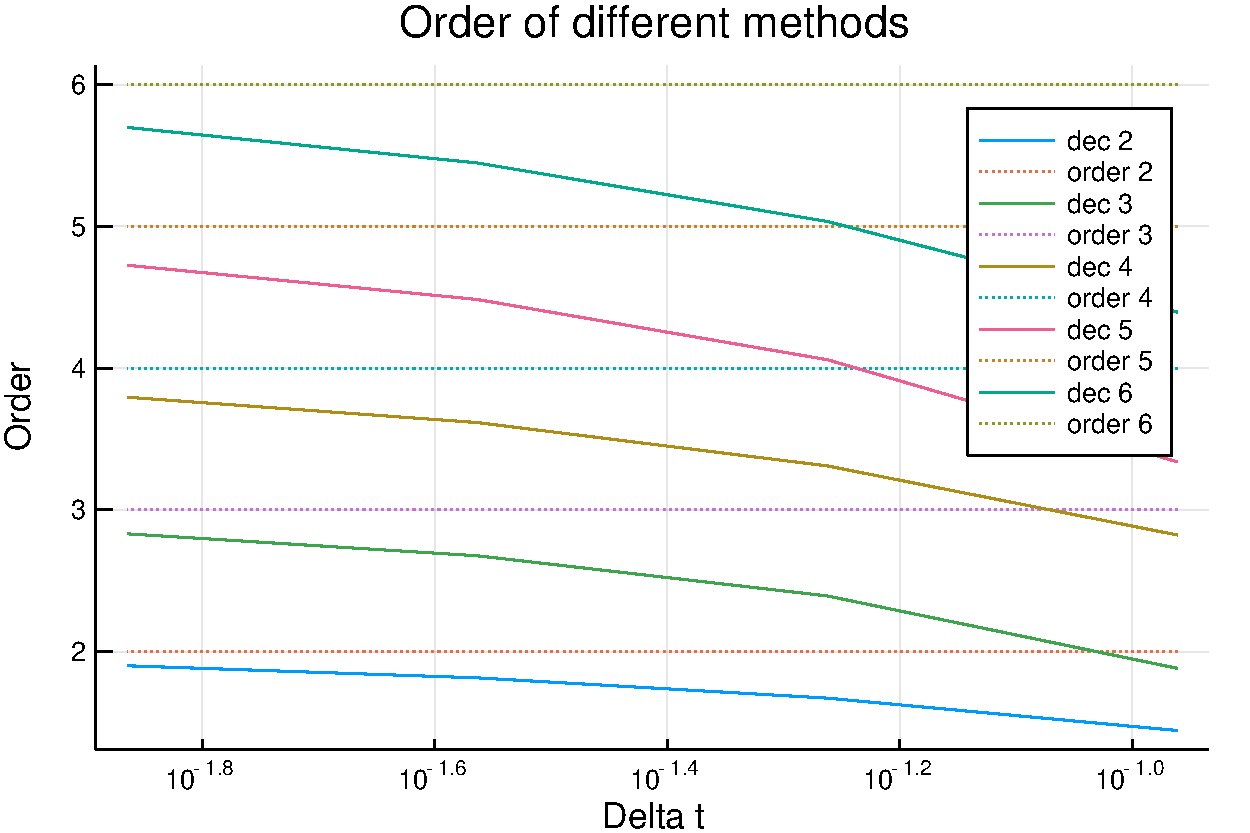
\includegraphics[width=0.48\textwidth]{images/LinearIntegralSlopesOrders26.pdf}
  \caption{ Second to sixth order error decay and slope of the errors
 }
  \label{fig:Linear_model_error}
\end{figure}

\end{frame}


\begin{frame}{Nonlinear test}
\begin{equation}\label{eq:nonlinear_test}
 \begin{cases}
  c_1'(t)&=-\frac{c_1(t)c_2(t)}{c_1(t)+1},\\
  c_2'(t)&= \frac{c_1(t)c_2(t)}{c_1(t)+1}-0.3c_2(t),\\
  c_3'(t)&=0.3c_2(t)
 \end{cases}
\end{equation}
with initial condition $\bc^0=(9.98,0.01,0.01)^T$. 

The PDS system in the matrix formulation can be expressed by 
\begin{equation*}
 p_{2,1}(\bc)=d_{1,2}(\bc)=\frac{c_1(t)c_2(t)}{c_1(t)+1}, \quad  p_{3,2}(\bc)=d_{2,3}(\bc)=0.3c_2(t)
\end{equation*}
and $p_{i,j}(\bc)=d_{i,j}(\bc)=0$ for all other combinations of $i$ and $j$. 

\end{frame}

\begin{frame}{Nonlinear test}
\begin{figure}[!htp]
\centering
    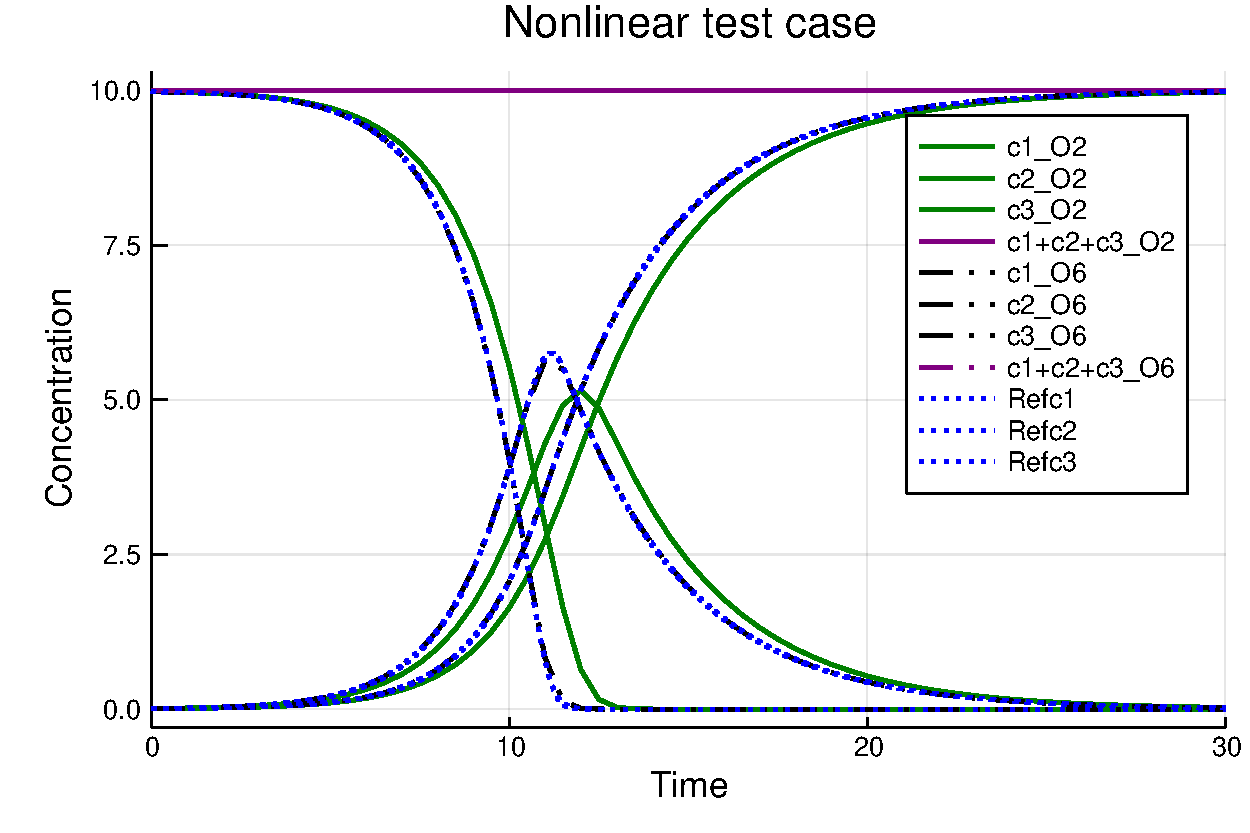
\includegraphics[height=0.7\textheight]{images/NonlinearWithReferenceSSPRK104.pdf}
 %   \includegraphics[width=0.45\textwidth]{Figures/Nonlinear/WithReference_DP.pdf}
  \caption{ Second order and sixth order methods together with the reference solution (SSPRK104)
 }
  \label{fig:Non_linear}
\end{figure}
\end{frame}

\begin{frame}{Nonlinear test: Convergence}
\begin{figure}[!htp]
\centering
    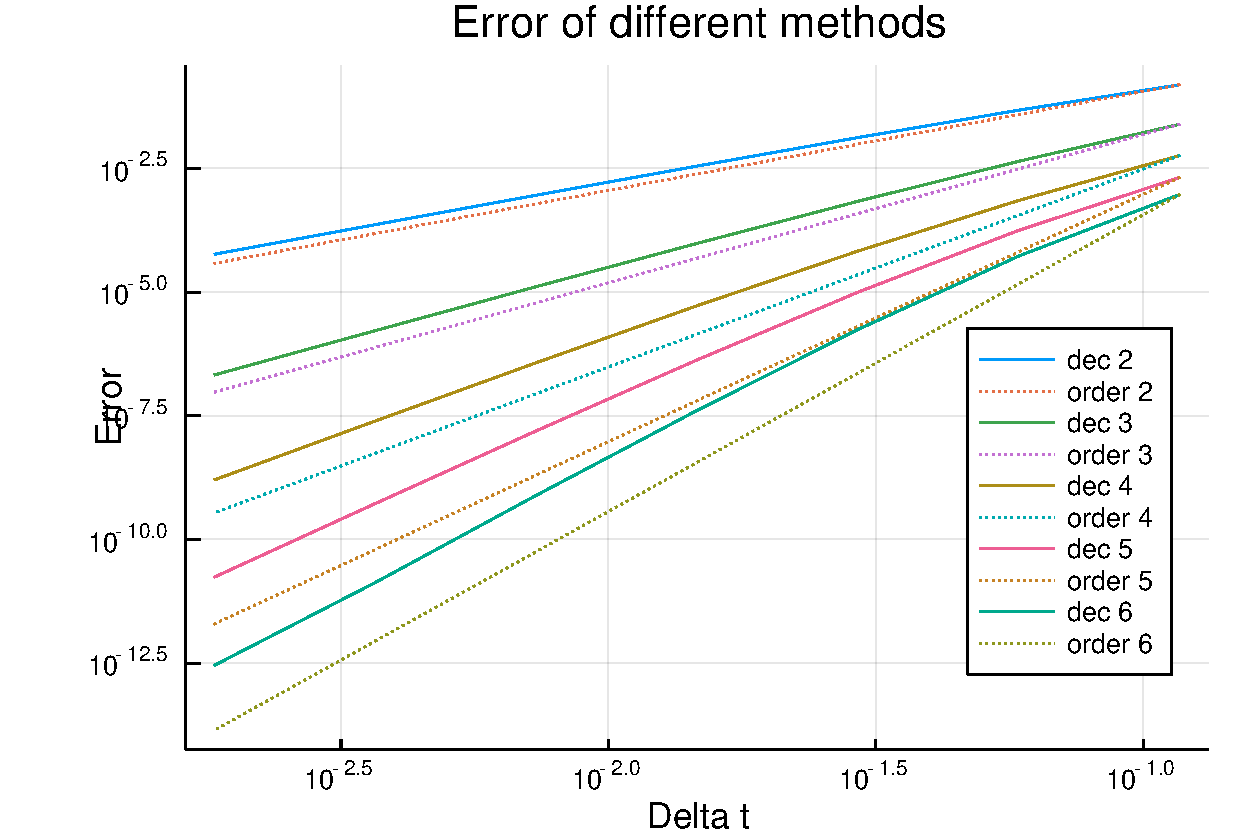
\includegraphics[width=0.48\textwidth]{images/NonlinearIntegralErrorOrders26.pdf}
    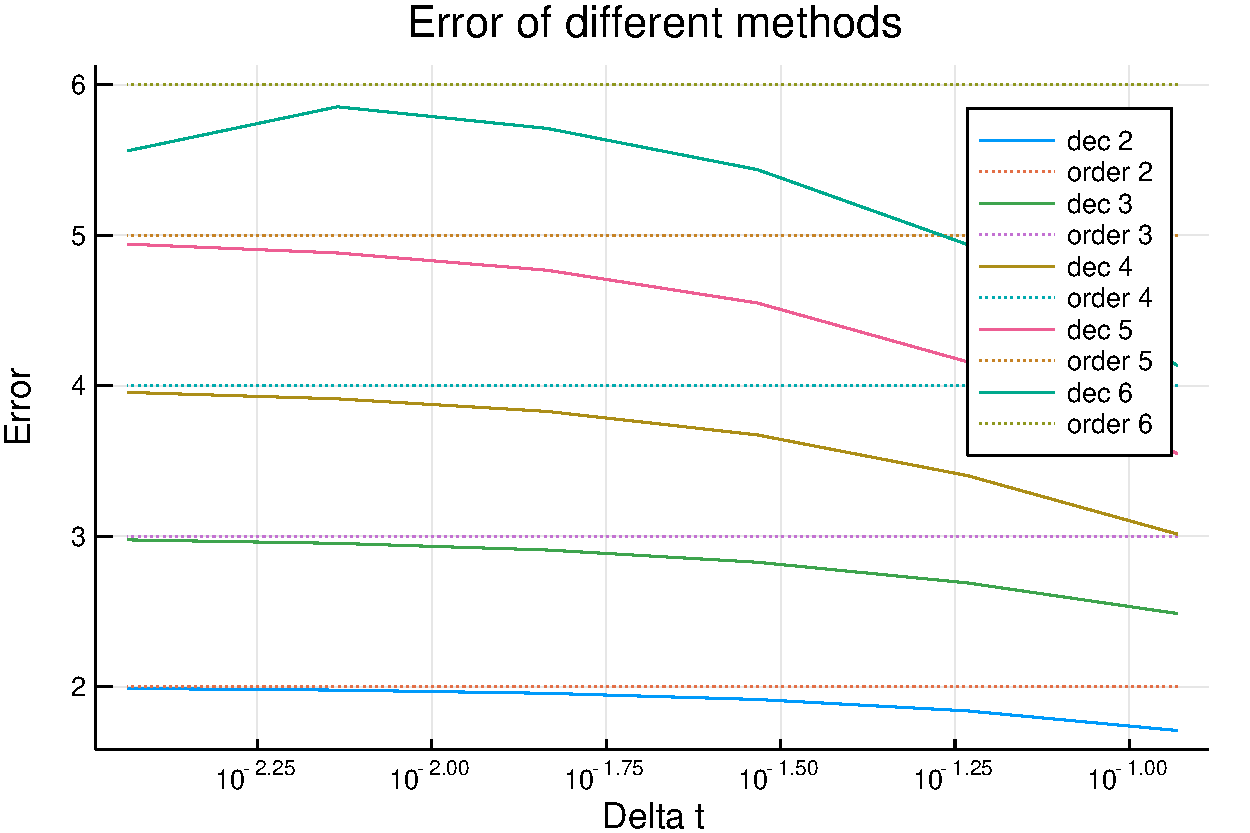
\includegraphics[width=0.48\textwidth]{images/NonlinearIntegralSlopesOrders26.pdf}
  \caption{ Second to sixth order error behaviors and slopes of the errors
 }
  \label{fig:Non_Linear_model_error}
\end{figure}


\end{frame}


\begin{frame}{SIRD}
	\begin{minipage}{0.35\textwidth}
		\begin{equation*}
		\begin{cases}
		d_tS = - \beta \frac{SI}{N}\\
		d_t I = \beta \frac{SI}{N} -\gamma I- \delta I \\
		d_t R = \gamma I\\
		d_t D = \delta I
		\end{cases}
		\end{equation*}
		Solved with mPDeC5
	\end{minipage} \hfill
	\begin{minipage}{0.63\textwidth}
	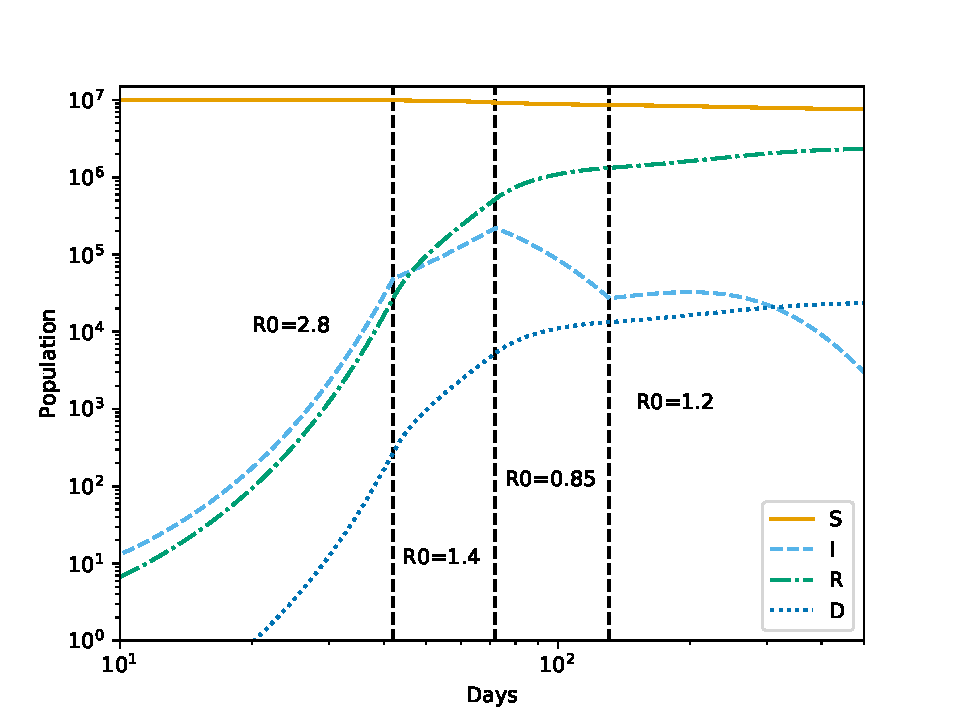
\includegraphics[height=0.8\textheight]{images/SIRsimul.pdf}
\end{minipage}
	
\end{frame}


\begin{frame}{Robertson test}
\begin{equation}\label{eq:Robertson}
 \begin{aligned}
  c_1'(t)&=10^4c_2(t)c_3(t)-0.04c_1(t)\\
  c_2'(t)&= 0.04c_1(t)-10^4c_2(t)c_3(t)-3\cdot 10^7c_2(t)^2\\
  c_3'(t)&=3\cdot 10^7c_2(t)^2
 \end{aligned}
\end{equation}
with initial conditions
$\bc^0=(1,0,0)$.

The time interval of interest is $[10^{-6}, 10^{10}]$.
The PDS for \eqref{eq:Robertson} reads
\begin{equation*}
\begin{split}
 & p_{1,2}(\bc)=d_{2,1}(\bc)=10^4c_2(t)c_3(t), \quad  
 p_{2,1}(\bc)=d_{1,2}(\bc)=0.04c_1(t),\\ 
 & p_{3,2}(\bc)=d_{2,3}(\bc)=3\cdot 10^7c_2(t)
\end{split}
\end{equation*}
and zero for the other combinations.

We use exponential timesteps to better catch the behaviour of the solution $\Delta t^n = 2\cdot \Delta t^{n-1}$.
\end{frame}

\begin{frame}{Robertson test}
\begin{figure}[!htp]
\center
    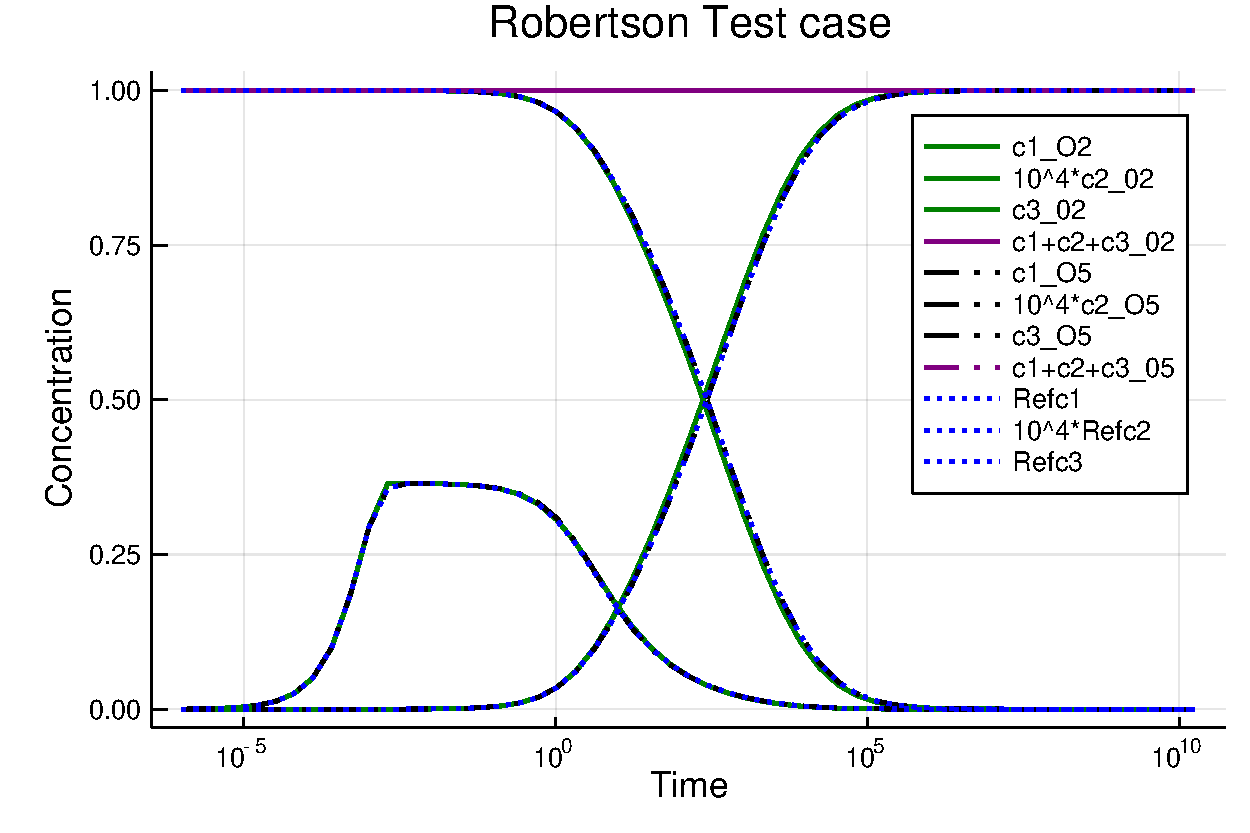
\includegraphics[height=0.7\textheight]{images/RobertsonOrder25.pdf}
  %  \includegraphics[width=0.45\textwidth]{Figures/Robertson/Solution_Order_2.pdf}
  \caption{ Second and fifth order solutions and references 
 }
  \label{fig:Robertson}
\end{figure}

\end{frame}

\begin{frame}{Application to Shallow Water equations}
	\begin{minipage}{0.48\textwidth}
		$$
		\begin{cases}
			\partial_t h  + \nabla \cdot (h \bu) = 0\\
			\partial_t \bu + \nabla \cdot ( h \bu \otimes \bu + g \frac{h^2}{2} \mathrm{I})= - g h \nabla b(\mathbf{x})
		\end{cases}
		$$
		\begin{itemize}
			\item	\href{https://davidetorlo.it/files/talks/mpdecsw_honom22.pdf}{Slides}\\
			\item	\href{https://davidetorlo.it/publication/2021-10-27-sw-mpdec}{Article post}				
		\end{itemize}
	\end{minipage}\hfill
	\begin{minipage}{0.48\textwidth}
		\begin{figure}
			\centering
			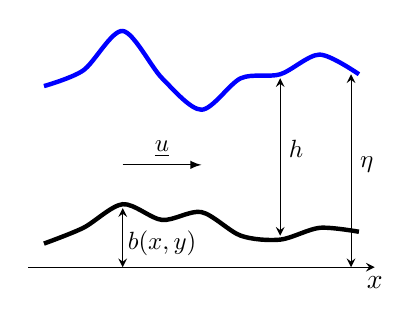
\begin{tikzpicture}
				
				\draw [-stealth] (-0.2,-0.3) -- (4.2,-0.3);
				\node [black,scale=1] at (4.2,-0.5) {$x$};
				
				\draw [stealth-stealth] (1,-0.3) -- (1,0.45);
				\node [black,scale=0.9] at (1.5,0) {$b(x,y)$};
				\draw [stealth-stealth] (3,0.1) -- (3,2.1);
				\node [black,scale=0.9] at (3.2,1.2) {$h$};
				\draw [stealth-stealth] (3.9,-0.3) -- (3.9,2.15);
				\node [black,scale=0.9] at (4.1,1.0) {$\eta$};
				
				\draw [-latex] (1,1) -- (2,1);
				\node [black,scale=0.9] at (1.5,1.2) {$\vec{u}$};
				
				\draw [black,ultra thick] plot [smooth] coordinates {(0,0) (0.5,0.2) (1,0.5) (1.5,0.3) (2,0.4) (2.5,0.1) (3,0.05) (3.5,0.2) (4,0.15)};
				\draw [blue, ultra thick]  plot [smooth] coordinates {(0,2) (0.5,2.2) (1,2.7) (1.5,2.1) (2,1.7) (2.5,2.1) (3,2.15) (3.5,2.4) (4,2.15)};
				
			\end{tikzpicture}
			\caption{Shallow Water Equations: definition of the variables.}\label{fig:SWE}
		\end{figure}
			
	\end{minipage}


	\begin{itemize}
		\item MPDeC Code: If you want to check out the code, it's really easy ($\sim 150$ lines), in Julia, on git.

		\url{https://git.math.uzh.ch/abgrall_group/deferred-correction-patankar-scheme}
		
		\item MPDeC Shallow Water code (Fortran)
		\url{https://github.com/accdavlo/sw-mpdec}
	\end{itemize}

\end{frame}

\end{document}




